\chapter{GLcode}          % chapter 1
\label{codechap}

\section{GL}
GL is a GPU based Ginzburg-Landau field simulator. It was designed to solve mesoscale problems which arised in superconductor design. To model the system accurately, we need to take into account the Ginzburg Landau function at a microscopic resolution. At the same time, the system size has to be large enough to encompass many vortex interactions and complicated non-superconducting architectures. Physical pinning defects are simulated as modulations of the superconductor's critical temperature. The simulation works by first integrating the GL equations forward in time, then solving the Poisson equiation to find the electric and magnetic fields. There are also noise correlation terms to simulate thermal effects~\cite{Sadovskyy14}.

\section{Results}
Being such a general code, there were many possible areas of study regarding this code. We found promissing results in two general areas, grids of inclusions and hyper-conducting funnels. We characterize these situations by looking at their responses to changes in voltage, magnetic field, and geometry. There is an important choice that we made when determining the critical current as there is a inherent hysteresis in the system. We had two options when ramping the current. It could either have been ramped up, Starting with no movement and pushing the current until the vortices became dislodged. The second option was to ramp the current down. That is start with moving vortices and slowly decrease the current until the vortices become lodged. In the end we went for the second option due to the dynamics of the system. Vortices tend to start out placed not according to the lowest energy state, but instead randomly according to whatever starting seed was selected. By forcing the vortices to move around first, we get a more natural state before the depinning current is found. In figure ~\ref{hysteresis} we quantitatively demonstrate the difference.

\begin{figure}[htbp]
\begin{center}
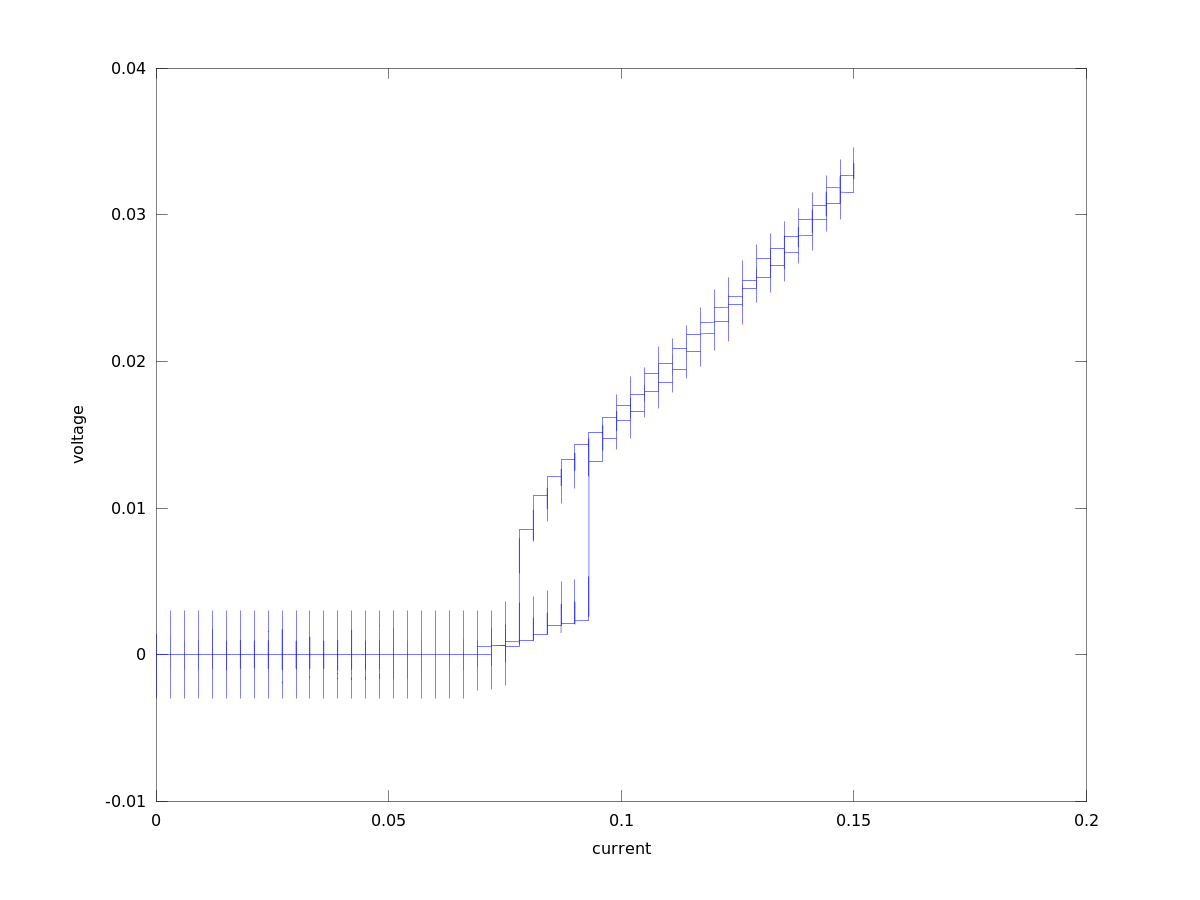
\includegraphics[scale=.50]{JvV.png}
\caption{ Overlapped are the current vs voltage for two systems, one with the current ramped up and one with the current ramped down. Upper one is the current being ramped down, while the lower one is the current ramped up.}
\label{hysteresis}
\end{center}
\end{figure}
 

\subsection{Grids}
Inclusions in the superconductive substrate can be used to contain vortices (up to a certain current). If these vortices do not move, then they are not draining energy from the system. The first thing we needed to show was that vortices preferred to be trapped in inclusions which were around the same size as they were. If the inclusion size is increased, we see that at some point we start to trap 2 vortices per inclusion. Trapping a vortex requires that the force due to external current and other vortices be less than the superconducting destruction force. The superconducting destruction force is due to the energy of a superconducting system below Tc Being lower than a non-superconducting system below Tc. The second effect we were looking for was vortex matching resistance. Vortices have quantized magnetic flux. This means that for a certain applied field, we can predict the number of vortices. If some vortices are moving and some are pinned, the moving ones will push on the pinned ones as they pass by. If instead we have as many vortices as we have inclusions, after a certain relaxation period, vortices will all be pinned and the system will be more stable. As shown in Fig.~\ref{HDF} we were able to show both of these effects. In the X direction, we see that the optimal radius for an inclusion is 2. In the Y direction, we see a sharp drop in critical current at m=1. This is because as soon as we are above the 1-to-1 ratio, we start to have rogue vortices which will move.

\begin{figure}[htbp]
\begin{center}
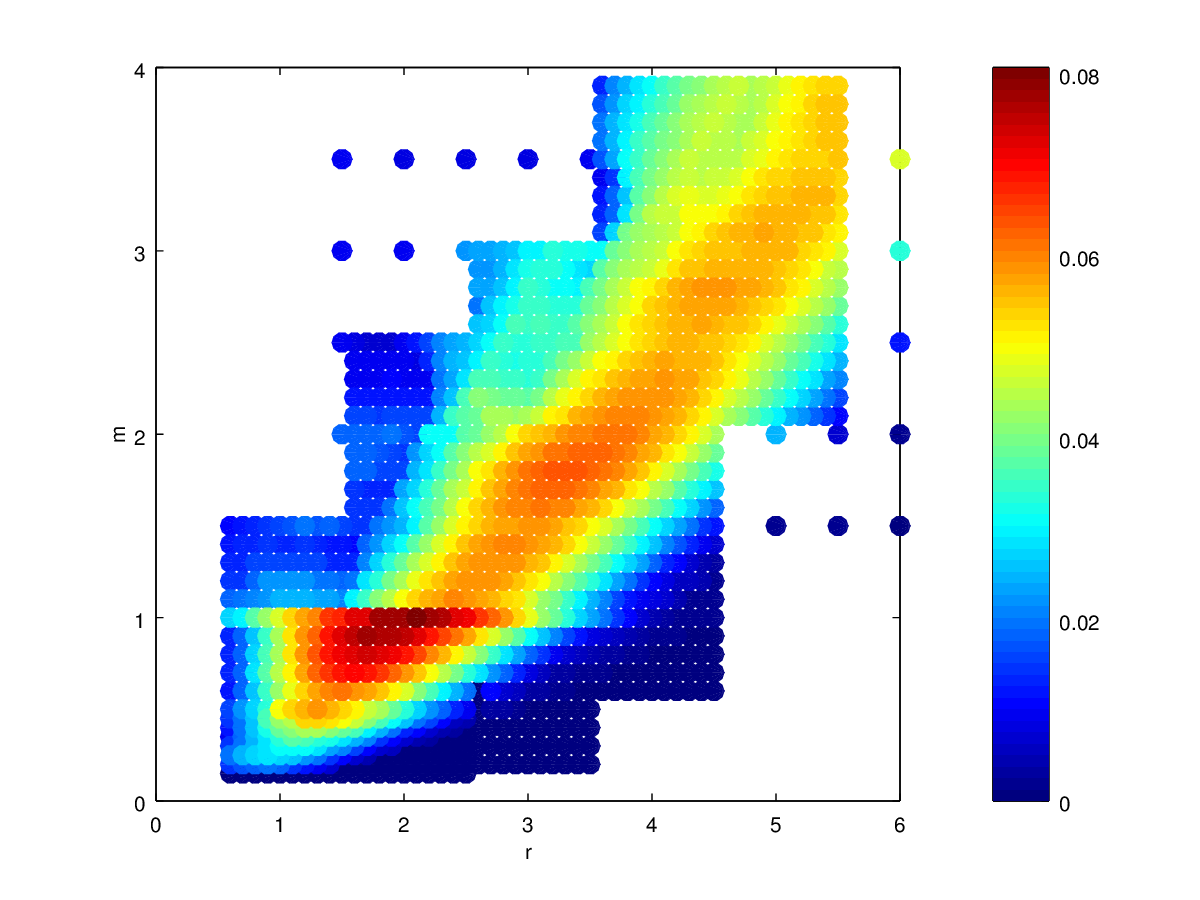
\includegraphics[scale=.50]{HDFinal.png}
\caption{ On the X-axis is the radius of each inclusion in the system. On the Y axis m is the ratio of number of vortices per inclusion. The colorbar stands for critical current. In other words, the redder a zone is, the better it holds on to vortices, the lower superconductive resistance it puts out.}
\label{HDF}
\end{center}
\end{figure}
 

\subsection{Funnels}
The same way that energy is gained when a vortex goes into a lower superconducting state, energy is lost if it tries to go into a higher superconducting state. Also, since more current can travel through the hyperconducting system, we get the opposite of the venturi effect. This also helps to keep vortices out. Using this logic, we created hyperconducting zones that can be used to guide vortices. Indeed, increasing the aperture size increases the ease of which the vortices can travel ~\ref{AvR}. 

\begin{figure}[htbp]
\begin{center}
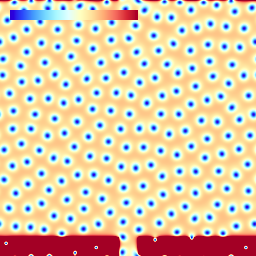
\includegraphics[scale=.50]{ratchetNoAngle.png}
\caption{ The amplitude of the complex order parameter. in yellow is the background superconductor, In red is the superconductor wall, and the blue dots are the vortices. In green is the parameter of interest. In this case, we have a flat obstruction which forces vortices through a narrow gap.}
\label{noAngle}
\end{center}
\end{figure} 

\begin{figure}[htbp]
\begin{center}
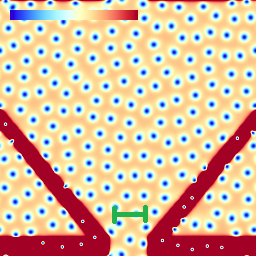
\includegraphics[scale=.50]{normalX.png}
\caption{ The amplitude of the complex order parameter. in yellow is the background superconductor, In red is the superconductor wall, and the blue dots are the vortices. In green is the parameter of interest. In this case it is the size of the aperture which was varied. }
\label{normalX}
\end{center}
\end{figure}

\begin{figure}[htbp]
\begin{center}
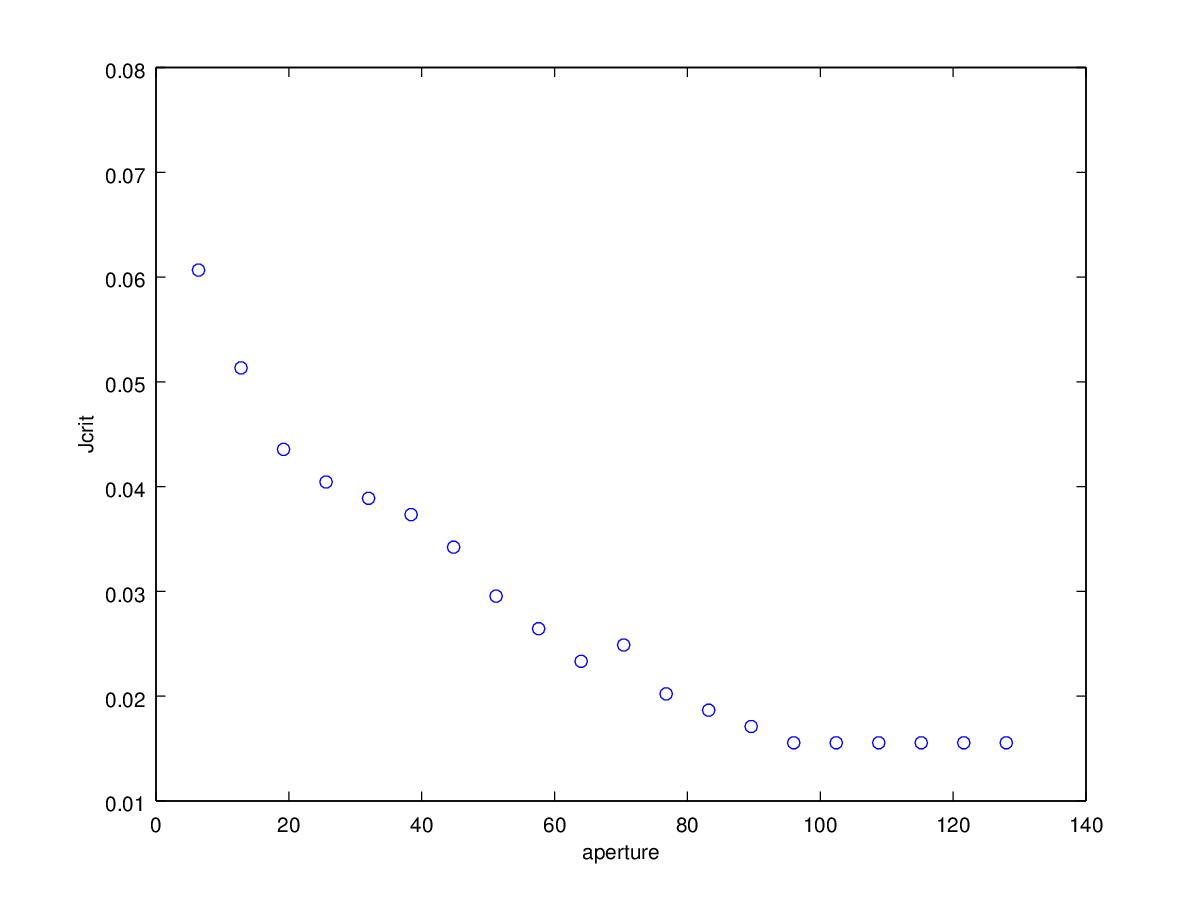
\includegraphics[scale=.50]{normalXscan.png}
\caption{ 50 values of aperture were run in this simulation. The resulting current was analyzed to find the critical current . As the aperture is increased, the ability to hold the vortices still is diminished. }
\label{normalXscan}
\end{center}
\end{figure}

\begin{figure}[htbp]
\begin{center}
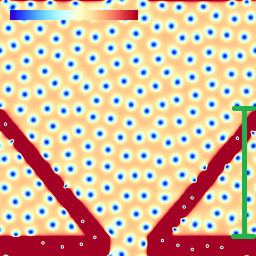
\includegraphics[scale=.50]{normalY.png}
\caption{ The amplitude of the complex order parameter. in yellow is the background superconductor, In red is the superconductor wall, and the blue dots are the vortices. In green is the parameter of interest. In this case it is the point on the Y-axis at which the funnel attaches and therefore the angle which varies. }
\label{normalY}
\end{center}
\end{figure}

\begin{figure}[htbp]
\begin{center}
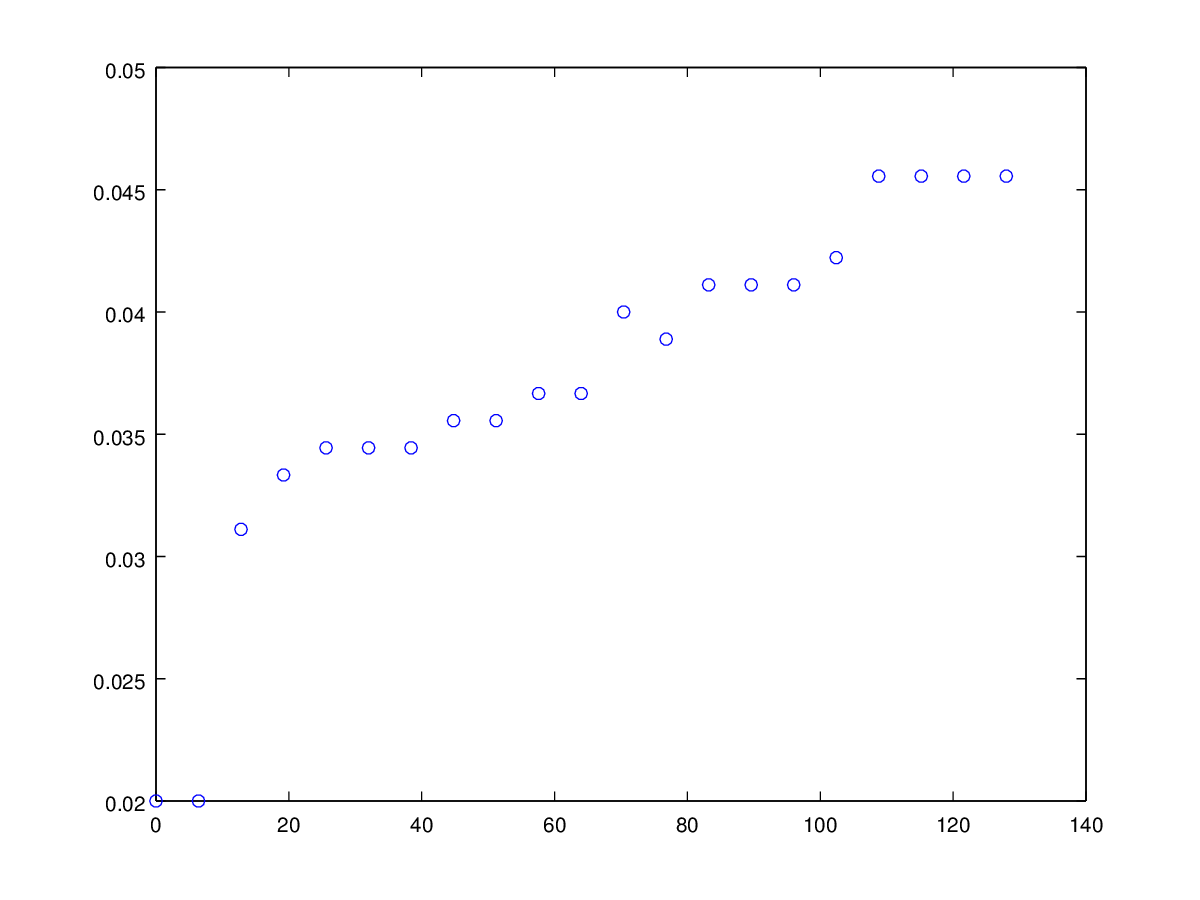
\includegraphics[scale=.50]{normalYscan.png}
\caption{ 50 values of aperture were run in this simulation. The resulting current versus voltage information was analyzed to find the critical current . As the aperture is increased, the ability to hold the vortices still is diminished. }
\label{normalYscan}
\end{center}
\end{figure}


\begin{figure}[htbp]
\begin{center}
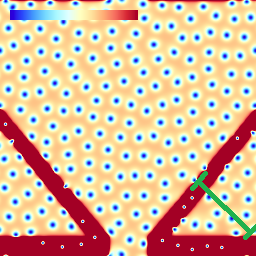
\includegraphics[scale=.50]{normalAngle.png}
\caption{ The amplitude of the complex order parameter. in yellow is the background superconductor, In red is the superconductor wall, and the blue dots are the vortices. In green is the parameter of interest. In this case the angle is held constant while the x and y attachments are varied. }
\label{normalAngle}
\end{center}
\end{figure}

\begin{figure}[htbp]
\begin{center}
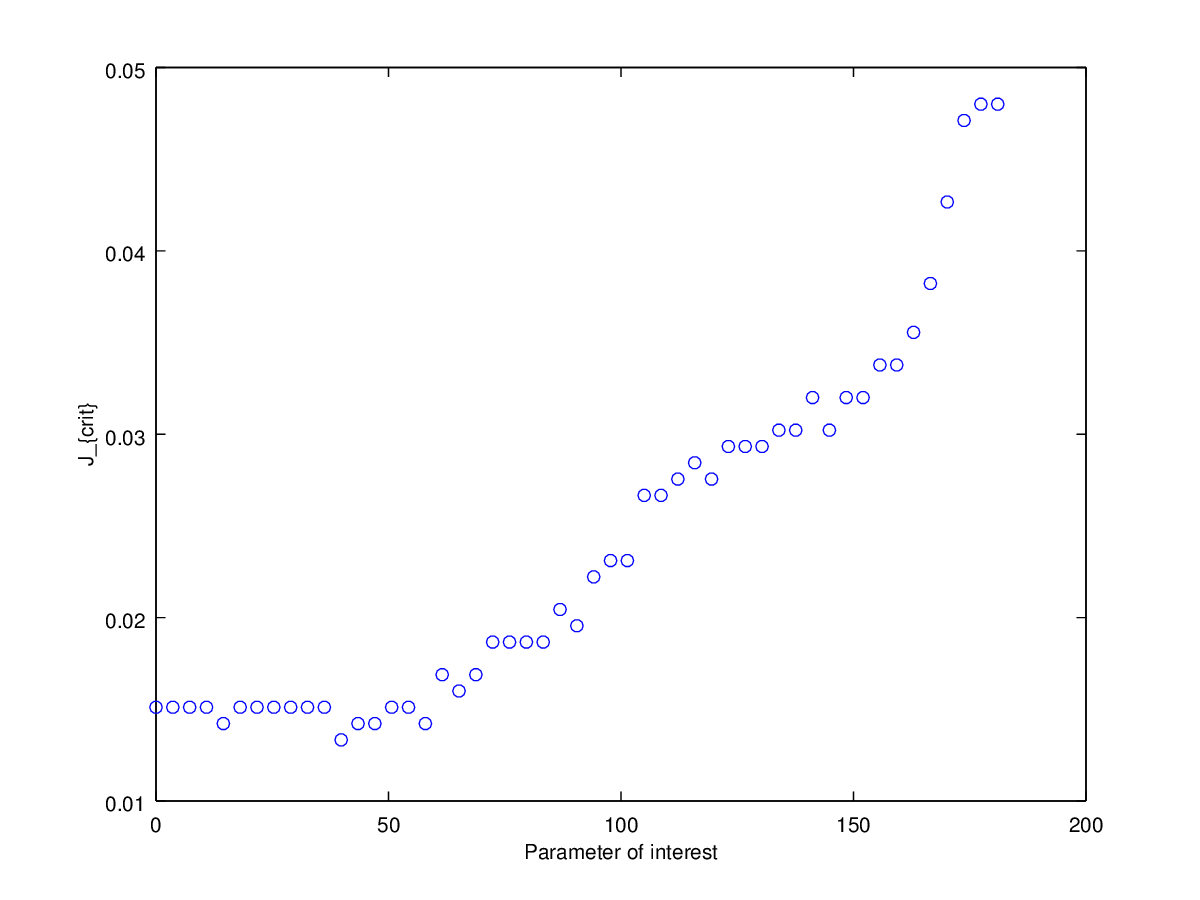
\includegraphics[scale=.50]{constantAngle.png}
\caption{ This is a scan of the parameter of interest versus the critical current. The x-postition and y-position of the funnel were moved uniformly as to keep the angle constant. }
\label{constantAngle}
\end{center}
\end{figure}


\begin{figure}[htbp]
\begin{center}
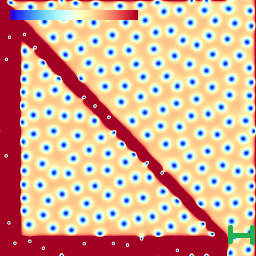
\includegraphics[scale=.50]{oneSidedDone.png}
\caption{ The amplitude of the complex order parameter. in yellow is the background superconductor, In red is the superconductor wall, and the blue dots are the vortices. In green is the parameter of interest. In this case it is the size of the aperture which was varied. }
\label{oneSidedX}
\end{center}
\end{figure}


\begin{figure}[htbp]
\begin{center}
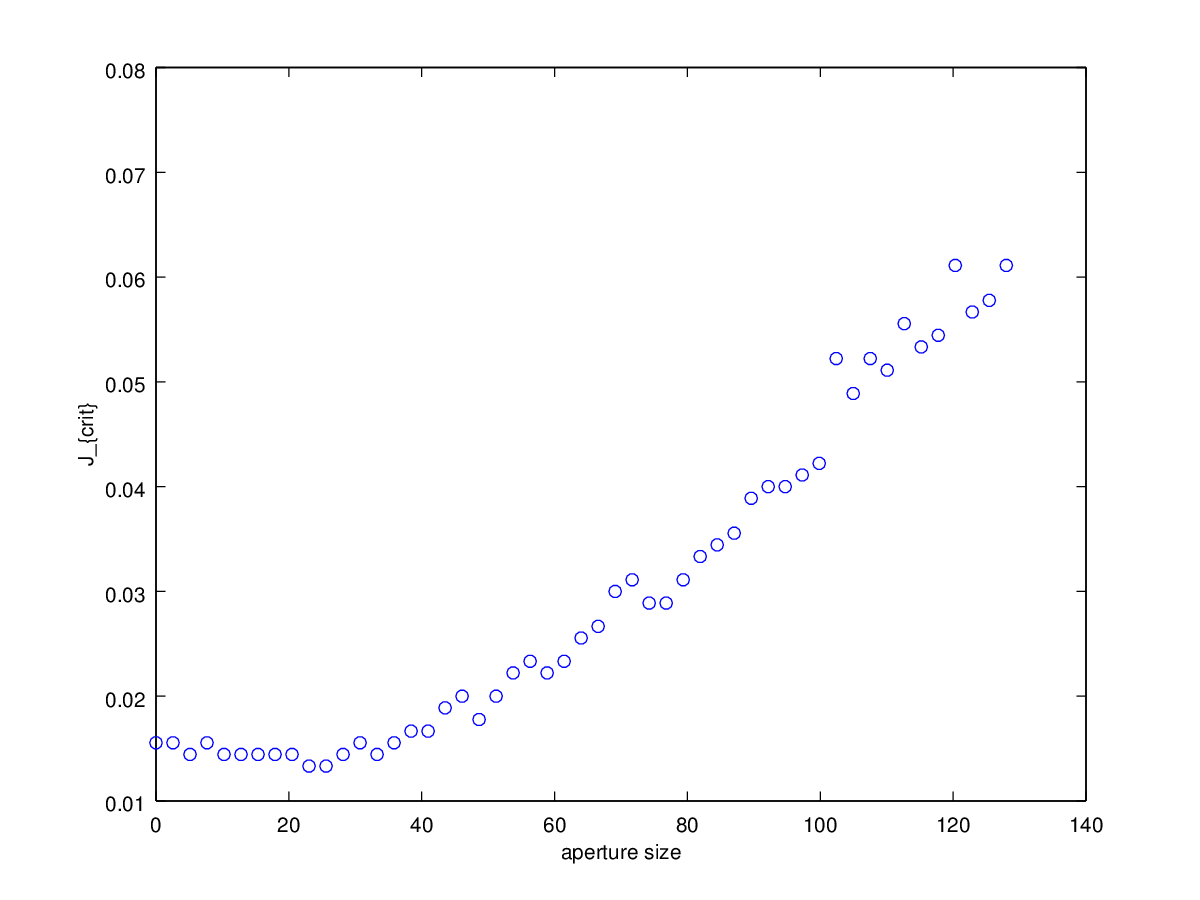
\includegraphics[scale=.50]{oneSidedAperture.png}
\caption{ 50 values of aperture were run in this simulation. The resulting current versus voltage information was analyzed to find the critical current . As the aperture size is increased, the vortices are less restrained. }
\label{normalYscan}
\end{center}
\end{figure}

\begin{figure}[htbp]
\begin{center}
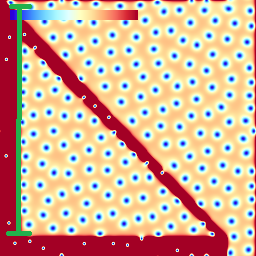
\includegraphics[scale=.50]{oneSidedY.png}
\caption{ The amplitude of the complex order parameter. in yellow is the background superconductor, In red is the superconductor wall, and the blue dots are the vortices. In green is the parameter of interest. In this case it is the point on the Y-axis at which the funnel attaches and therefore the angle which varies.}
\label{oneSidedY}
\end{center}
\end{figure}

\begin{figure}[htbp]
\begin{center}
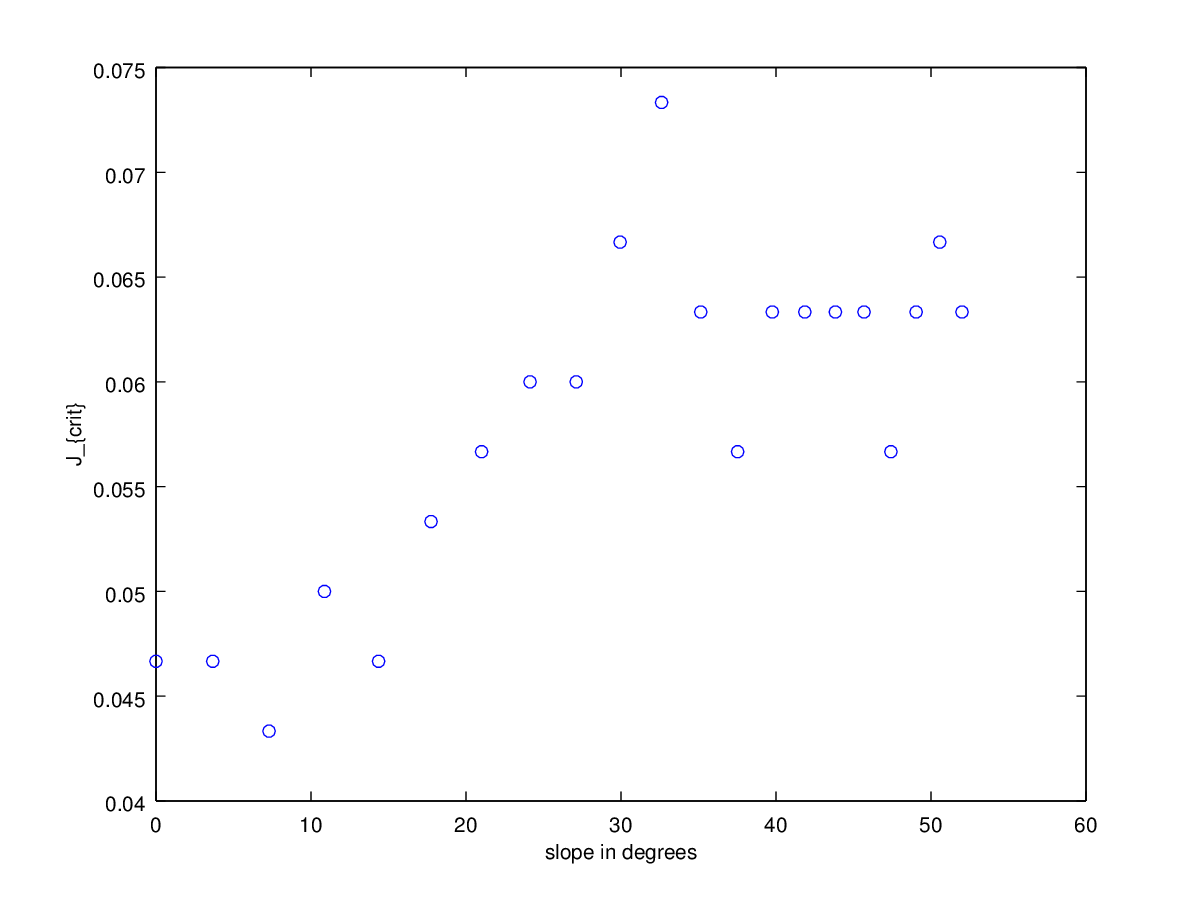
\includegraphics[scale=.50]{oneside-angle-Scan.png}
\caption{ 50 values of aperture were run in this simulation. The resulting current versus voltage information was analyzed to find the critical current . As the one slope is increased, the jamming effect becomes more pronounced. }
\label{normalYscan}
\end{center}
\end{figure}

\begin{figure}[htbp]
\begin{center}
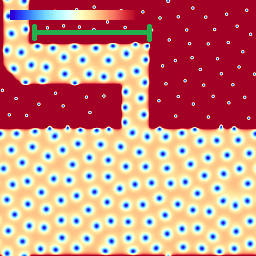
\includegraphics[scale=.50]{oneKinkDone.png}
\caption{ The amplitude of the complex order parameter. in yellow is the background superconductor, In red is the superconductor wall, and the blue dots are the vortices. In green is the parameter of interest. In this case it is the length of the "turn" which is being varied.}
\label{oneSidedY}
\end{center}
\end{figure}

\begin{figure}[htbp]
\begin{center}
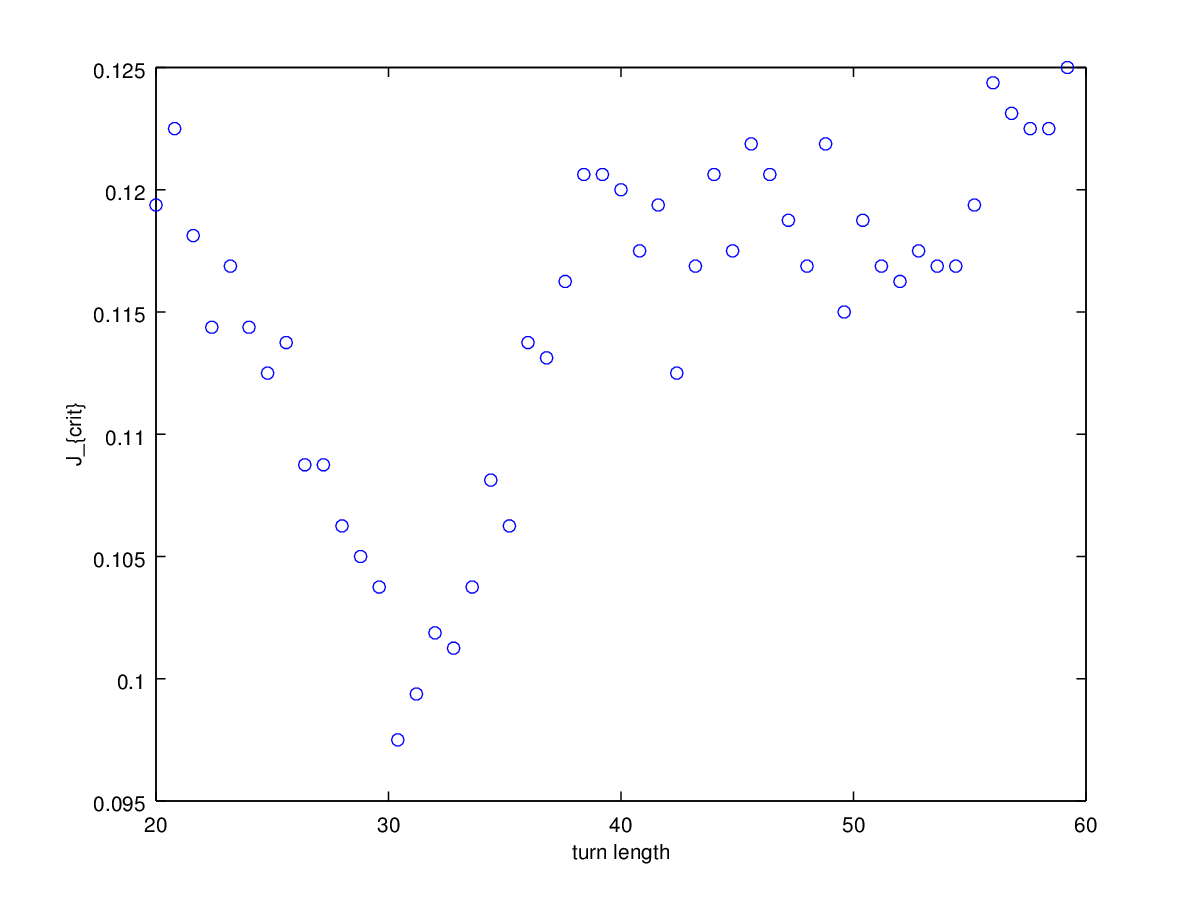
\includegraphics[scale=.50]{kinkScan.png}
\caption{ 50 values of the turn length were run in this simulation. The resulting current versus voltage information was analyzed to find the critical current .  }
\label{normalYscan}
\end{center}
\end{figure}



\begin{figure}[htbp]
\begin{center}
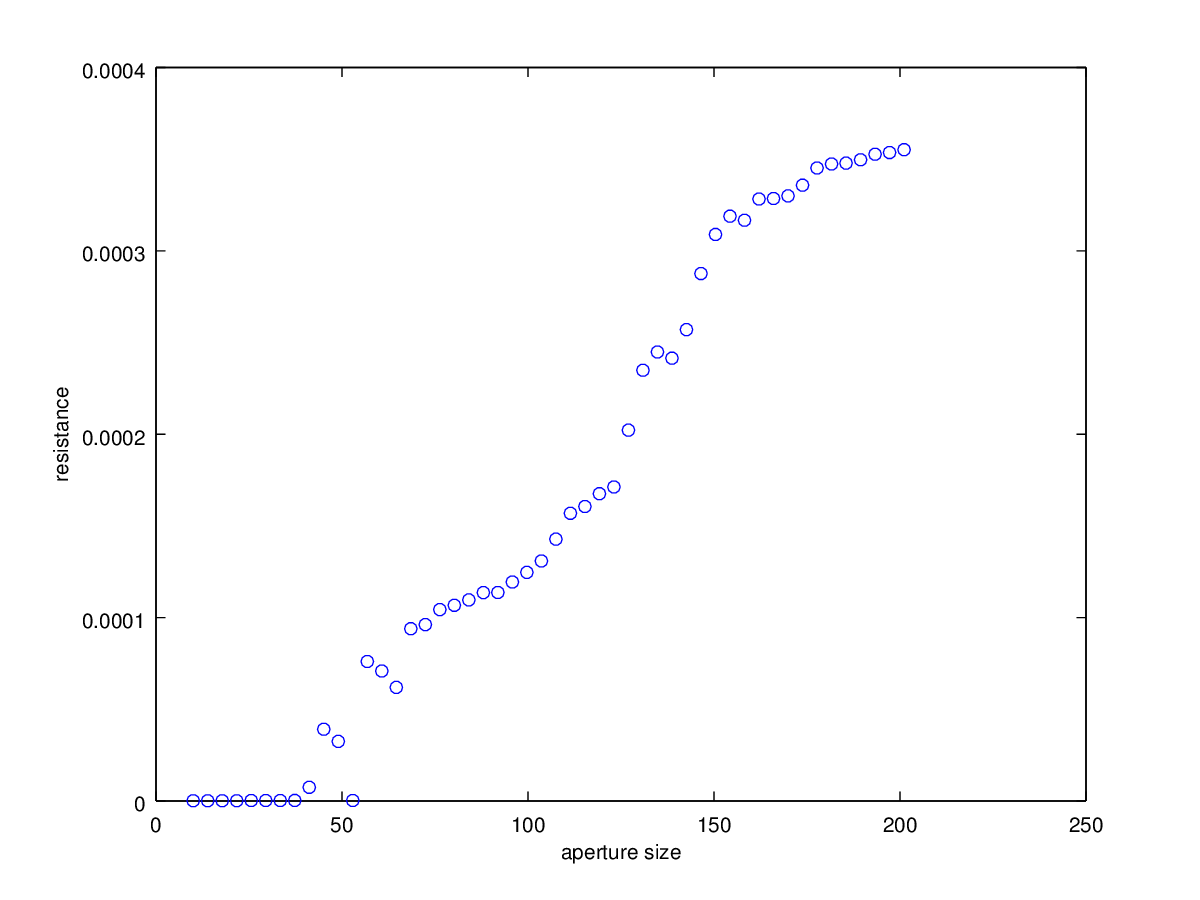
\includegraphics[scale=.50]{AvR.png}
\caption{ We can also study how the aperture size hampers vortex movement once they have already been depinned. This is a resistance plot of the constant y-position funnel. On the X axis is the size of the aperture, Y axis is the superconductive resistance. }
\label{AvR}
\end{center}
\end{figure}



